\begin{multicols}{2}
\section*{Objetivo General}
\normalsize{Determinar experimentalmente la aceleración gravitacional \(g\) a partir de un experimento de caída libre}\\
\section*{Objetivos específicos}
%\normalsize{
\begin{enumerate}
    \item Medir desplazamientos para un objeto en caída libre.
    \item Representar el movimiento del objeto mediante la construcción de gráficos que faciliten su análisis.
    \item Determinar la aceleración gravitacional g experimentalmente.
\end{enumerate} 
%}\\
\section*{Referentes conceptuales}
El ejemplo más conocido de un movimiento con aceleración constante es la caída de un cuerpo bajo la influencia de la atracción gravitacional terrestre, bajo la aproximación que la distancia de caída es pequeña comparada con el radio terrestre, e ignorando los efectos debidos a la rotación de la Tierra y a la fuerza de ficción presentada por el aire.

Esta aceleración constante es dirigida hacia el centro de la Tierra, se denota con la letra g y se conoce como aceleración gravitacional y su valor en la superficie terrestre es de aproximadamente $9.77 m/s^2$ reportada para Bogotá en 1997.

\begin{center}
    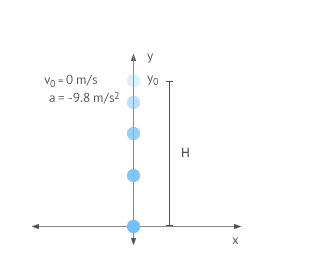
\includegraphics[scale=0.7]{fig/caida-libre.png}
\end{center}

La ecuación 3.1 de movimiento, permite obtener la posición de un cuerpo en función del tiempo para una aceleración constante. Si el movimiento es completamente vertical su velocidad aumenta.


\[y(t) = y_o + v_o \cdot t  - \dfrac{g t^2}{2} \]

Donde $y(t)$ representa la posición, $g$ la aceleración y $t$ el tiempo. Si el cuerpo “cae” desde el reposo $(v_o = 0)$ en un tiempo inicial $t_o = 0$. Si se define como $y_o = 0$ el punto desde donde se deja caer la ecuación anterior se reduce a la ecuación:
\[ y(t) = - \dfrac{g t^2}{2} \]

\section*{Actividades Previas}   
\begin{enumerate}
\item Tras observar el vídeo \url{https://www.youtube.com/watch?v=Y4AJo-Ana70}. La relación y la diferencia entre las constantes G y g es: ...
\item  En el punto más alto de una caída libre la velocidad en y siempre es 0 porque ... pero la aceleración siempre va a ser igual a la gravedad porque ...
\item Diferencias y semejanzas que pueda tener un objeto en caída libre y un objeto lanzado de forma vertical hacia arriba: ... .
\item El primero en medir el valor de la aceleración gravitacional g fue ... (Galileo) ... \textit{descripcion del proceso ...}.

\end{enumerate}
    
\section*{Materiales de Laboratorio}  
\begin{enumerate}
    \item Un celular con la aplicación PhyPhox establecida en el modo cronómetro acústico
    \item 30 globos
    \item Un flexómetro
\end{enumerate}

\section*{Procedimiento}
\begin{enumerate}
    \item Ingresar a la aplicación y elegir el cronómetro acústico.

    \item En modo simple, se estableció el valor del “Umbral” a 0.2 y el “Retraso Mínimo” a 0.1
    
    \item Elegir un área que cuente con una altura moderada y en la cual se tenga una superficie que pueda ser impactada, en este laboratorio se eligió la terraza de una casa. 
    
    \item Ubicar el móvil sobre una base sólida de forma que el micrófono no se encuentre obstruido y pueda tener mayor sensibilidad auditiva.
    
    \item Al explotar la bomba, se producirá el sonido que indica el comienzo de la caída del objeto (inicia el cronómetro),inmediatamente el objeto cae.
    
    \item Tomar tres mediciones de tiempo (Medida 1, Medida 2 y Medida 3) para 5 alturas diferentes y registrar los datos en la tabla 1.
    
    \item Cambiar el objeto por uno de mayor o menor peso, repetir los puntos 8 al 9, y registrar los datos en la tabla 2.
\end{enumerate}

\section*{Resultados}
%Tabla 1
\begin{figure}[H]
    \centering
    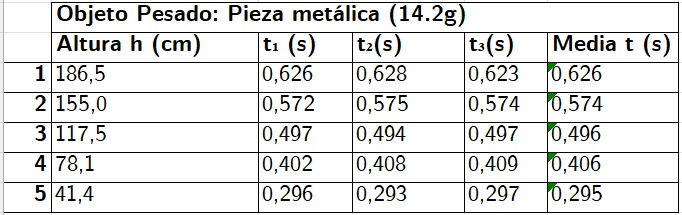
\includegraphics[scale=0.3]{fig/Tabla1-ObjetoPesado.png}
    \caption{...}
\end{figure}

%Tabla 2
\begin{figure}[H]
    \centering
    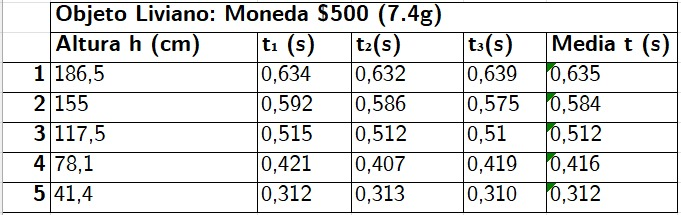
\includegraphics[scale=0.3]{fig/Tabla2-ObjetoLiviano.png}
    \caption{...}
\end{figure}

\section*{Análisis cuantitativo y cualitativo} 
\textbf{Gráficas}
        \begin{figure}[H]
            \centering
            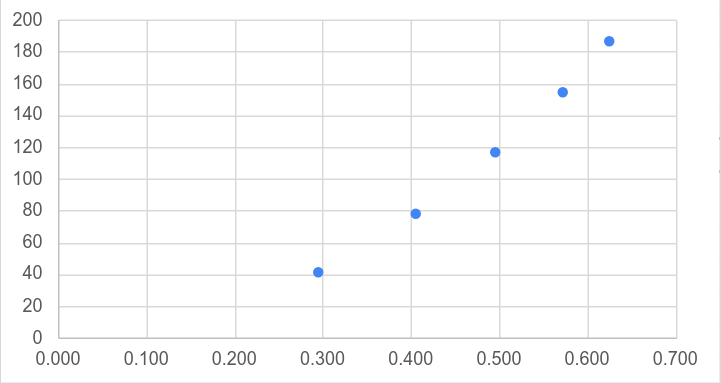
\includegraphics[scale=0.5]{fig/objPesado-Altura-Tiempo.png}
            \caption{Gráfica de Altura vs Tiempo para Objeto Pesado}
        \end{figure}
        
        \begin{figure}[H]
            \centering
            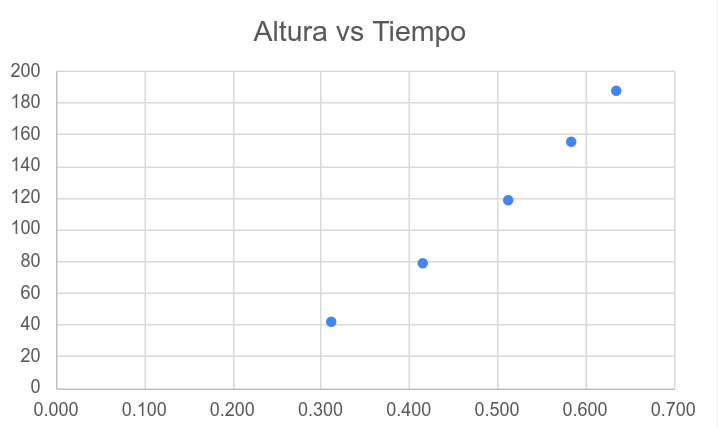
\includegraphics[scale=0.5]{fig/objLiviano-Altura-Tiempo.png}
            \caption{Gráfica de Altura vs Tiempo para Objeto Liviano}
        \end{figure}
\textbf{Gráficas}
...
%Tabla 3
\begin{figure}[H]
    \centering
    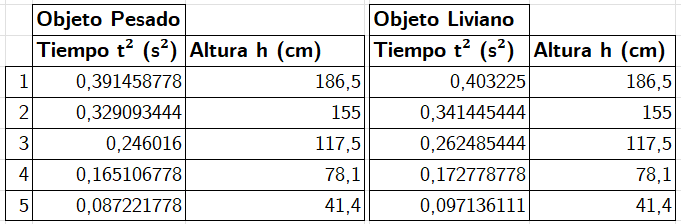
\includegraphics[scale=0.5]{fig/Tabla3-TiempoCuadrado.png}
    \caption{...}
\end{figure}


\textbf{Regresión por mínimos cuadrados}
\begin{figure}[H]
    \centering
    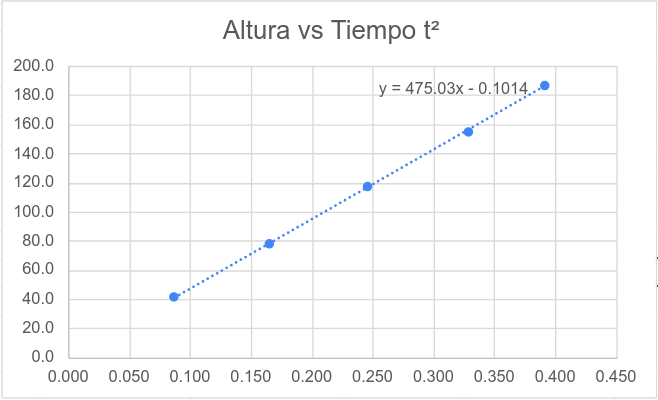
\includegraphics[scale=0.5]{fig/objPesado-Altura-TiempoCuadrado.png}
    \caption{Gráfica de Altura vs Tiempo Cuadrado para Objeto Pesado}
\end{figure}

\begin{figure}[H]
    \centering
    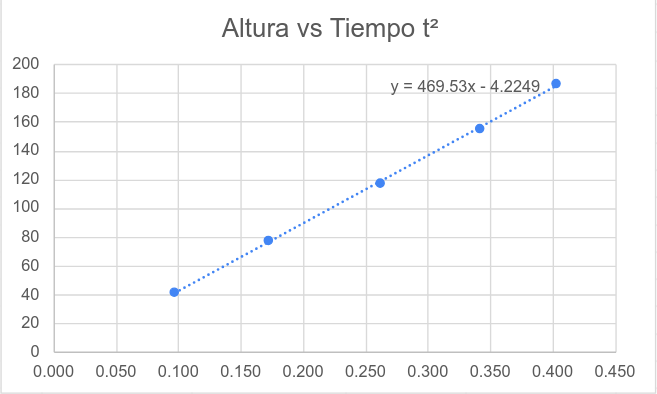
\includegraphics[scale=0.5]{fig/objLiviano-Altura-TiempoCuadrado.png}
    \caption{Gráfica de Altura vs Tiempo Cuadrado para Objeto Liviano}
\end{figure}

\textbf{Determinación de la aceleración gravitacional g} \\
Mediante las ecuaciones obtenidas en la regresión por mínimos cuadrados:

\begin{enumerate}
    \item $y = 475.03x - 0.1014$
    \item $y = 469.53x - 4.2249$
\end{enumerate}


Se sabe que $x$ es el tiempo al cuadrado $t^2$, $y$ es la altura. Para calcular la aceleración gravitacional g se tiene que: \\
\[ y(t) = - \dfrac{g t^2}{2} \] \\
\[ y = m t^2\] \\

\begin{enumerate}
    \item Para el objeto pesado: \[m = \dfrac{g}{2} = 475.0 \ cm/s^2 = 4.75 \ m/s^2\] \\ \[g = 9.5 \ m/s^2\]
    \item Para el objeto liviano:\[m = \dfrac{g}{2} = 469.5 \ cm/s^2 = 4.695 \ m/s^2\] \\ \[g = 9.39 \ m/s^2\]
\end{enumerate}



\section*{Conclusiones} 
\begin{enumerate}
    \item Cosas a tener en cuenta: ...
    \item Sugerencias para mejorar el experimento: ...
\end{enumerate}
\section*{Referencias bibliográficas}
\small{
$\cdot$ Alonso M. y Finn E. J., “Física” Vol. I, Ed. Addison-Wesley Iberoamericana (1986). \\ 
$\cdot$ Tipler, P.A. Física Vol 1. Ed Reverté, México, (1985).\\
$\cdot$ Sears, F.- Zemansky, M.Física Universitaria I. Ed Pearson, México (1999).\\
$\cdot$ Serway, R. Física I para ciencias e ingeniería. Ed Thomson, México (2005)
}
\end{multicols}